% Owner: Sergiu
\section{Performance model}
\label{sec:model}

\paragraph{Which model.} BFS does almost no floating-point operations, so a normal roofline
in FLOP/byte~\cite{roofline} does not make sense here. If we use examined edges as the unit of
work instead, the arithmetic intensity is only 1.49 million edges per \SI{179}{MB}, so about
\num{0.008} edges per byte. The ECM model needs a loop that always does the same work with
predictable data transfers, so that in-core time and transfer time can be added. BFS has early
exits that depend on the data, atomic operations, and the work changes in every level, so
ECM does not fit either. We therefore used the information exchange model from the lectures:
we count how many bytes have to be moved and how many random accesses have to be waited
for, based on the work we counted and not on the size of the graph. Then we compute two
lower bounds, one for bandwidth and one for latency, with parameters that we measured
ourselves:
\begin{align*}
T_\text{bw}(p)  &= \frac{Q}{\min(p\,B_1,\;B_\text{all})}, &
T_\text{lat}(p) &= \frac{N_\text{rand}\; L_\text{DRAM}}{\text{MLP}\cdot p}, &
T_\text{model}(p) &= \max(T_\text{bw}, T_\text{lat}).
\end{align*}
Here $Q$ is the amount of data of one search, $B_1$ and $B_\text{all}$ are the STREAM triad
bandwidth with one thread and with all threads, $N_\text{rand}$ is the number of random cache
line accesses, $L_\text{DRAM}$ is the latency of a dependent load at \SI{1}{GB}, and MLP is
the number of misses that one core can have open at the same time (Little's law).
$T_\text{model}$ is a lower bound: it ignores synchronisation and assumes that all data comes
from main memory.

\paragraph{Parameters.} $Q$ and $N_\text{rand}$ come from the edge counts of
Section~\ref{sec:app} (Table~\ref{tab:traffic}). In bottom-up, every checked vertex costs at
least one cache line of its neighbour list (usually the first neighbours are enough). In
top-down, every examined edge costs 4 bytes for the neighbour ID and one random cache line of
\texttt{parent}. The loops over \texttt{parent} (\SI{4}{B} per vertex), the CSR index
(\SI{8}{B} per vertex) and the bitmaps are sequential. We measured the MLP with up to 32
pointer chases at the same time on one core. On the laptop the time per load goes down from
\SI{262}{ns} with one chain to \SI{17}{ns} with 16 chains, so MLP $= 15.7$. This fits the 16
L1 miss status handling registers (MSHRs, also called fill buffers) of a Golden Cove core,
which limit the number of open misses. On Hábrók the time per load goes down from
\SI{101}{ns} to \SI{4.65}{ns} with 32 chains, so MLP $= 21.7$.

\begin{table}[ht]
\centering\small
\caption{Modelled amount of data of one \texttt{kron20} search.}
\label{tab:traffic}
\begin{tabular}{@{}lr@{}}
\toprule
Part & MB per search \\
\midrule
\texttt{InitParent} (read index, write \texttt{parent}) & 12.6 \\
Bottom-up loops over all vertices, $2.5\times(12n + n/8)$ & 31.8 \\
Bottom-up: one neighbour line per checked vertex ($1.66$M $\times$ \SI{64}{B}) & 106.2 \\
Top-down: $0.29$M edges $\times$ (\SI{4}{B} + one random \SI{64}{B} line) & 19.5 \\
Conversions and last loop & 8.7 \\
\midrule
Total $Q$ & \textbf{178.8} \\
Random line accesses $N_\text{rand}$ & 1.95 M \\
\bottomrule
\end{tabular}
\end{table}

\paragraph{Model against measurement.} Table~\ref{tab:model} and Figure~\ref{fig:model}
compare the model with the measured times.
\begin{table}[ht]
\centering\small
\caption{Model bounds and measured median (threads bound).}
\label{tab:model}
\begin{tabular}{@{}lrrrrrr@{}}
\toprule
Machine & $p$ & $T_\text{bw}$ [ms] & $T_\text{lat}$ [ms] & $T_\text{model}$ [ms] & measured [ms] & ratio \\
\midrule
Laptop & 1 & 14.6 & 46.7 & 46.7 & 56.5 & 1.21 \\
Laptop & 8 & 11.3 & 5.8 & 11.3 & 8.4 & 0.74 \\
Hábrók & 1 & 5.2 & 8.9 & 8.9 & 24.9 & 2.81 \\
Hábrók & 48 & 0.55 & 0.18 & 0.55 & 1.38 & 2.52 \\
Hábrók & 128 & 0.55 & 0.07 & 0.55 & 3.53 & 6.46 \\
\bottomrule
\end{tabular}
\end{table}

\begin{figure}[ht]
\centering
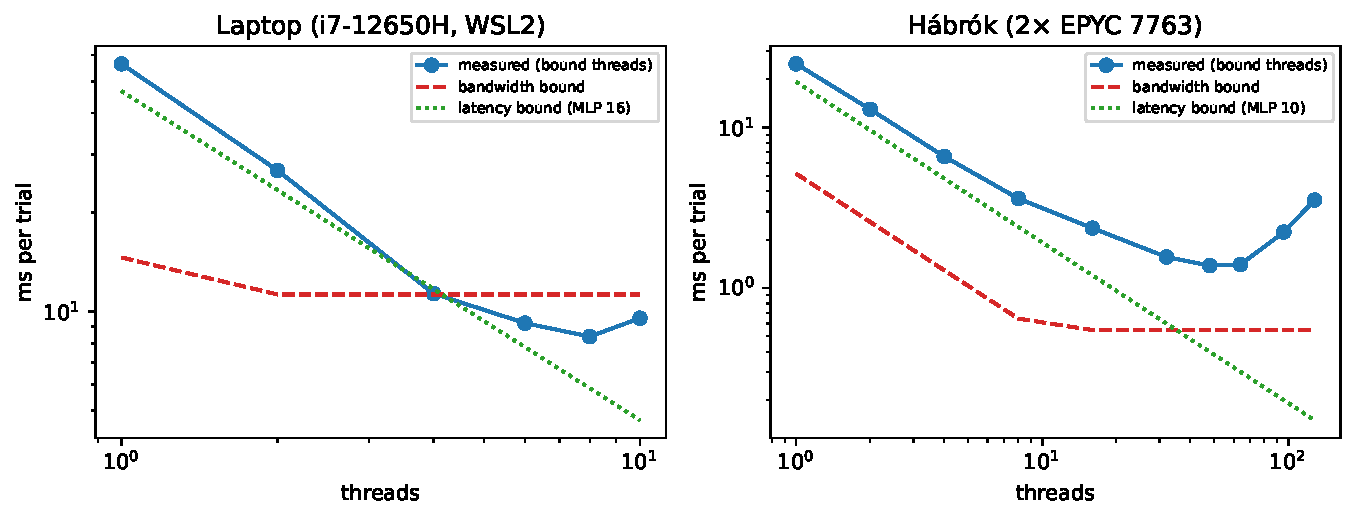
\includegraphics[width=0.9\linewidth]{figures/model.pdf}
\caption{Measured time per search (threads bound) with the bandwidth and latency bounds of
the model.}
\label{fig:model}
\end{figure}

We see three different cases:
\begin{enumerate}
  \item \textbf{One thread: limited by latency.} On both machines $T_\text{lat}$ is larger than
        $T_\text{bw}$, so one core cannot have enough misses open to use the bandwidth. On
        the laptop the measured time is \SI{21}{\percent} above the latency bound. On Hábrók it
        is 2.8 times the bound. This means the BFS only keeps about 7.7 misses open
        ($N_\text{rand} L_\text{DRAM} / T$), while the core could keep 21.7. Every checked
        vertex is a chain of loads that depend on each other (\texttt{parent[u]}, then the
        index, then the neighbour, then the bitmap word), so the out-of-order window only sees
        a few vertices at the same time. On the laptop the latency is much higher, so this
        limit is less visible there. To improve the model, we would have to use the MLP that
        BFS can really reach instead of the maximum of the core.
  \item \textbf{Laptop with all threads: limited by bandwidth.} With 8 threads the latency
        bound is below the bandwidth bound of \SI{11.3}{ms}. The measured \SI{8.4}{ms} is even
        \SI{26}{\percent} faster than this bound. Moving all \SI{179}{MB} from main memory in
        \SI{8.4}{ms} would need \SI{21}{GB/s}, which is more than the \SI{15.9}{GB/s} of
        STREAM, so part of the data comes from the \SI{24}{MiB} L3. \texttt{parent}
        (\SI{4}{MB}), the bitmaps and part of the index fit there. The laptop is at its
        bandwidth limit, which explains why more threads do not help
        (Figure~\ref{fig:scaling}).
  \item \textbf{Hábrók with many threads: neither bound.} Both bounds go down to about
        \SI{0.5}{ms}, but the best measured time is \SI{1.38}{ms} (2.5 times the bound), and
        with 128 threads it is 6.5 times the bound. The missing time is synchronisation
        (about ten barriers per search with up to 128 threads), unbalanced work, and coherence
        traffic between the two sockets. None of these are in a bandwidth and latency model.
        This explains why the Hábrók node is only 3 times faster than the laptop. It also
        shows that on Hábrók we should reduce the number of threads or the synchronisation,
        not the memory traffic.
\end{enumerate}

\paragraph{Attainable performance.} If we write the bound as GTEPS ($m/T_\text{model}$), the
laptop can reach \SI{1.4}{GTEPS} when all data comes from main memory. Because of the L3 we
already reach \SI{1.87}{GTEPS}, so there is not much more to gain without reducing $Q$. On
Hábrók the bound is about \SI{28}{GTEPS} for \texttt{kron20}, and our best result is
\SI{11.4}{GTEPS}. So Hábrók still has room, but only for optimisations that reduce
synchronisation, place the threads and data better, or reduce $Q$ with better locality.
